\section{Historical development and the literature landscape}\label{sec:history}
\subsection{A short history}
\paragraph{Origins (1830s--1950s).} Duhamel's memoir of 1837 \citep{Duhamel1837} established the stress--strain--temperature relation that still bears his name (with Neumann's later contribution): the stress depends on strain and on the temperature increment through an expansion coefficient. The dynamic coupling appeared much later. Biot \citep{Biot1956} showed that the classical thermoelastic equations follow from the thermodynamics of irreversible processes with a Rayleigh-type dissipation function, and Danilovskaya \citep{Danilovskaya1950} solved the thermal shock of an elastic half-space, in the uncoupled approximation. Chadwick and Sneddon \citep{ChadwickSneddon1958} analysed plane waves in the coupled theory; Chadwick's chapter \citep{Chadwick1960} became the standard reference for the dynamical theory; compact textbook accounts followed \citep{Boley1960,Nowacki1975,Carlson1972}. The core results of that period are that the coupled longitudinal wave is attenuated and dispersed, that shear waves decouple in isotropic media, and that the thermal disturbance is a diffusive wave. Zener's earlier analysis of thermoelastic internal friction in vibrating reeds \citep{Zener1937} had already shown the same relaxation behaviour from a different direction.

\paragraph{Finite-speed heat conduction (1940s--1970s).} The conceptual starting point is Cattaneo's 1948 note \citep{Cattaneo1948} and Vernotte's independent discussion \citep{Vernotte1958}, which add a relaxation term to Fourier's law, making the heat equation hyperbolic. Experimental support from low-temperature solids, namely second sound in solid helium and in sodium fluoride \citep{Ackerman1966,Jackson1970}, and a kinetic theory of phonon hydrodynamics \citep{GuyerKrumhansl1966,GuyerKrumhansl1966II,Chester1963}, supplied physical contexts in which heat actually propagates as a wave. Lord and Shulman \citep{Lord1967} then built Cattaneo's law into a complete thermoelastic theory, and Green and Lindsay \citep{Green1972} proposed a different extension with two relaxation times in the constitutive relations. The relation between these theories and thermodynamics was the subject of extensive discussion; reviews are \citep{Chandrasekharaiah1986,Joseph1989,Joseph1990}.

\paragraph{Energy-based theories (1990s).} Green and Naghdi \citep{Green1991,GreenGN1992,Green1993} introduced a family of three theories (types I, II, III) based on an entropy balance rather than an entropy inequality for the heat flux, in which the thermal displacement plays the role of a potential. Type II is a nondissipative theory with undamped thermal waves; type III contains classical damping and thermal waves. Uniqueness and stability theory developed around these \citep{Chandrasekharaiah1996}.

\paragraph{Lagging models (1995--2010).} Tzou \citep{Tzou1995,Tzou1997} proposed that the heat flux and the temperature gradient are separated by delay times, giving the dual-phase-lag (DPL) model; Roy Choudhuri \citep{RoyChoudhuri2007} added a third lag associated with the thermal displacement. These models quickly spread because Taylor expansion of the lag equation gives a differential equation of finite order whose parameters can be chosen to fit data, and the stability and thermodynamic admissibility of those truncations has been studied extensively \citep{Quintanilla2003DPL,Chirita2016,Tibullo2017,vanDerMerwe2021}.

\paragraph{Nonlocal, fractional and memory-dependent extensions (1970s--present).} Eringen's nonlocal elasticity \citep{Eringen1972,Eringen1983,Eringen2002} and its thermoelastic extension \citep{Eringen1974} predate the generalized heat theories but converge with them in micro- and nanosystems; gradient elasticity \citep{Aifantis1992,Aifantis2003,Askes2006,Askes2011} is the other main enrichment. Fractional calculus entered heat conduction through the Caputo derivative \citep{Caputo1967}, was developed into fractional thermoelasticity \citep{Povstenko2004,Povstenko2007,Povstenko2009,Povstenko2011Cattaneo,Povstenko2016,Sherief2010Fractional,Ezzat2011}, and was joined by the memory-dependent derivative of Wang and Li \citep{Wang2011,Wang2021}. Two-temperature theories \citep{ChenGurtin1968,Youssef2006} and their hyperbolic variants \citep{Prasad2020,Alzahrani2020,Bassiouny2020} introduced a distinction between conductive and thermodynamic temperature.

\paragraph{Mathematical thermoelasticity of third order (2010s).} The Moore--Gibson--Thompson (MGT) equation, which arose in nonlinear acoustics \citep{MooreGibson1960}, was studied systematically as an evolution problem \citep{MarchandMcDevittTriggiani2012,LasieckaWang2015MGT,DellOroLasieckaPata2016MGT,DellOroPata2016Viscoelasticity} and then brought into thermoelasticity by Quintanilla \citep{Quintanilla2019,Bazarra2021MGTradial}, producing a model that fits the template of Section~\ref{sec:framework-link}.

\paragraph{Multiphysics and structure (1960s--present).} Micropolar and microcontinuum theories \citep{Eringen1966a,TauchertClausAriman1968,Eringen1999}, materials with voids \citep{Nunziato1979,Cowin1983,Iesan1986}, thermopiezoelectricity \citep{Mindlin1974Thermopiezo,Nowacki1978,Chandrasekharaiah1984}, and thermoelastic diffusion and magneto-thermoelasticity extended the mechanical content, usually with the heat law as an independent module.

\begin{figure}[t]\centering
\resizebox{\linewidth}{!}{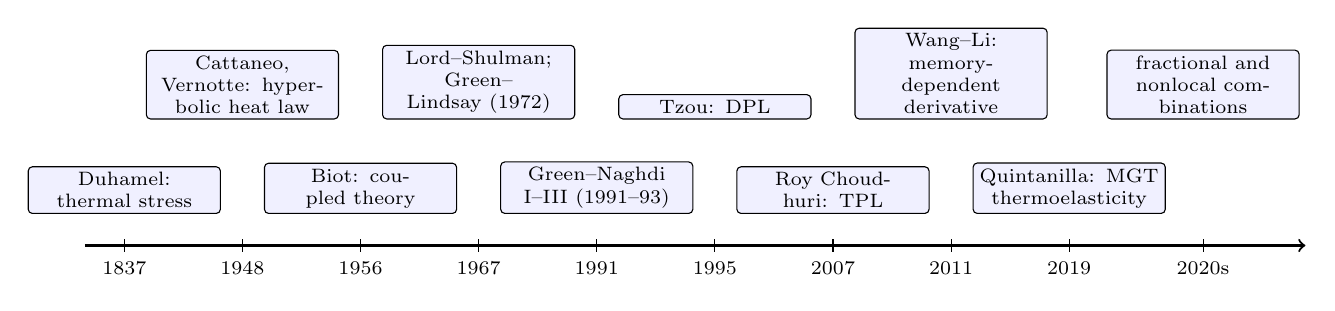
\begin{tikzpicture}[x=1cm,y=1cm,every node/.style={font=\scriptsize},
 ev/.style={draw,rounded corners=1.5pt,fill=blue!6,align=center,inner sep=2pt,text width=2.3cm}]
\draw[->,thick] (0,0)--(15.5,0);
\foreach \x/\l in {0.5/1837,2.0/1948,3.5/1956,5.0/1967,6.5/1991,8.0/1995,9.5/2007,11.0/2011,12.5/2019,14.2/2020s}{\draw (\x,0.08)--(\x,-0.08); \node[below] at (\x,-0.08) {\l};}
\node[ev,above] at (0.5,0.4) {Duhamel: thermal stress};
\node[ev,above] at (2.0,1.6) {Cattaneo, Vernotte: hyperbolic heat law};
\node[ev,above] at (3.5,0.4) {Biot: coupled theory};
\node[ev,above] at (5.0,1.6) {Lord--Shulman; Green--Lindsay (1972)};
\node[ev,above] at (6.5,0.4) {Green--Naghdi I--III (1991--93)};
\node[ev,above] at (8.0,1.6) {Tzou: DPL};
\node[ev,above] at (9.5,0.4) {Roy Choudhuri: TPL};
\node[ev,above] at (11.0,1.6) {Wang--Li: memory-dependent derivative};
\node[ev,above] at (12.5,0.4) {Quintanilla: MGT thermoelasticity};
\node[ev,above] at (14.2,1.6) {fractional and nonlocal combinations};
\end{tikzpicture}}
\caption{Milestones in the theory of thermoelastic waves. Dates are those of the cited original publications (Cattaneo 1948, Vernotte 1958, Biot 1956, Lord--Shulman 1967, Green--Lindsay 1972, Green--Naghdi 1991--1993, Tzou 1995, Roy Choudhuri 2007, Wang--Li 2011, Quintanilla 2019).}\label{fig:timeline}
\end{figure}

\subsection{A map of the contemporary literature}
The recent literature on wave problems in thermoelastic and multiphysics media can be sorted along three largely independent axes: the \emph{heat-flux law}, the \emph{constitutive enrichment} (nonlocal, gradient, microstructural, multiphysics), and the \emph{problem type} (plane waves, surface waves, reflection and transmission, transient response). A typical paper chooses one entry on each axis and computes dispersion curves or response histories. \Cref{tab:streams} lists representative works from our reference list by problem type; the sorting is editorial and many papers appear in more than one row.

\begin{table}[t]\centering\small
\caption{Representative literature by problem type and constitutive enrichment (selection from the reference list; classification by the titles and stated subjects of the works).}\label{tab:streams}
\begin{tabularx}{\textwidth}{@{}p{3.2cm}X@{}}\toprule
Problem type & Representative works\\\midrule
Plane waves, stability, dispersion & Prasad--Kumar \citep{Prasad2020}; Tiwari--Kumar (nonlocal TPL) \citep{Tiwari2021}; van der Merwe--van Rensburg (modal comparison of heat laws) \citep{vanDerMerwe2021}; Sarkar et al.\ (nonlocal type II) \citep{Sarkar2019}.\\
Surface waves & Biswas (porous nonlocal, orthotropic; piezothermoelastic layer) \citep{Biswas2020a,Biswas2020}; Tung (nonlocal piezoelastic Rayleigh) \citep{Tung2019}; Gupta et al.\ (nonlocal piezo-semiconductor Rayleigh wave) \citep{Gupta2024}; Aldandani et al.\ \citep{Aldandani2026}; Ivanov--Savova (energy flux of surface waves) \citep{IvanovSavova1991}.\\
Reflection at free or insulated boundaries & Das et al.\ \citep{Das2008}; Kalkal et al.\ (nonlocal micropolar with rotation) \citep{Kalkal2020}; Singh--Guha (piezothermoelastic fibre-reinforced) \citep{Singh2020b}; Yadav et al.\ \citep{Yadav2023}; Gupta et al.\ \citep{Gupta2024a}; Singh et al.\ (flexoelectric) \citep{Singh2020c}; Jiao et al.\ (flexomagnetic) \citep{Jiao2024}.\\
Interfaces and energy partition & Barak et al.\ \citep{Barak2023,Barak2023IJP,Barak2023JTS,Barak2023MMMS}; Gupta--Kumar \citep{Gupta2023IJNMF,Gupta2023Energy}; Kumar et al.\ \citep{Kumar2023PhysScr,Kumar2019,Kumar2022,Kumar2024,Kumar2024a,Kumar2025,KumarKansal2017,Kumar2018}; Fu--Wei (micropolar imperfect interface) \citep{Fu2013}; Liu et al.\ (graded piezoelectric) \citep{Liu2020}.\\
Transient response, rods, bodies & Singh--Pal \citep{Singh2019,Singh2020a}; Biswas \citep{Biswas2019}; Sur et al.\ \citep{Sur2019,Sur2025}; Bayones et al.\ \citep{Bayones2021}; Li et al.\ (laser pulse, bilayer) \citep{Li2019}; Abouelregal \citep{Abouelregal2023,Abouelregal2020,Abouelregal2020a}; Lata et al.\ \citep{Lata2020}.\\
Damping in resonators & Yang et al.\ (DPL damping in nonlocal nanoplates) \citep{Yang2021}; Kumar--Devi (couple stress plates) \citep{Kumar2017}.\\
Fractional and memory models & Povstenko \citep{Povstenko2004,Povstenko2009,Povstenko2011Cattaneo,Povstenko2016}; Sherief et al.\ \citep{Sherief2010Fractional}; Ezzat--El-Karamany \citep{Ezzat2011}; Wang--Li \citep{Wang2011,Wang2021,WangLi2025IV}; Yu et al.\ \citep{Yu2024}; Bachher--Sarkar \citep{Bachher2019}.\\
Size effects & Eringen \citep{Eringen1972,Eringen1983}; Aifantis \citep{Aifantis1992}; Askes--Aifantis \citep{Askes2006,Askes2011}; Maranganti--Sharma \citep{Maranganti2006,Maranganti2007}; Lazar--Agiasofitou \citep{Lazar2022}; Zang et al.\ \citep{Zang2014}; Li et al.\ \citep{Li2018}.\\
Variational and uniqueness theory & Marotti de Sciarra \citep{Marotti2013}; Srivastava--Mukhopadhyay \citep{Srivastava2026}; Chandrasekharaiah \citep{Chandrasekharaiah1996}; Chiri\c{t}\u{a} et al.\ \citep{Chirita2016,Tibullo2017}.\\
\bottomrule\end{tabularx}
\end{table}

\subsection{Recurrent observations from the literature}
Reading across these streams, we note patterns that shape the rest of this review.
\begin{itemize}
\item \textbf{The heat law and the elastic enrichment are treated as independent modules.} Most interface and surface-wave papers combine one of several heat laws with one of several enrichments, so the dispersion relations differ only through $G(s)$ and through the elastic operator. This is why a unified treatment is possible and why a limit-checking discipline matters.
\item \textbf{Energy ratios and amplitude ratios dominate the reflection literature.} The interface papers cited above report energy ratios, whose sum must equal one in a lossless setting. A sum different from one is therefore a diagnostic of either dissipation, an error in the flux definition, or both; Section~\ref{sec:interfaces} discusses this check in detail.
\item \textbf{Parameter values are rarely tied to measurements.} Lags and fractional orders are typically assigned convenient values, so many figures demonstrate a model rather than a material.
\item \textbf{The thermodynamic status of the Taylor-expanded models is delicate.}

\begin{summarybox}[Summary]
The historical line runs Fourier (parabolic) $\to$ Cattaneo/vernotte (flux relaxation) $\to$ Lord--Shulman $\to$ Green--Lindsay $\to$ Green--Naghdi types I--III $\to$ dual-phase-lag $\to$ three-phase-lag $\to$ Moore--Gibson--Thompson $\to$ fractional and memory-dependent laws. Each step adds one modelling ingredient (relaxation time, second temperature, thermal displacement, lag on temperature gradient, inertia term, memory kernel). Recurrent pitfalls: unmeasured lag parameters, Taylor truncation passed off as exact, mode-flux sums mistaken for energy conservation, GN-III confused with a finite-speed theory.
\end{summarybox} The papers of Chiri\c{t}\u{a} and co-workers \citep{Chirita2016,Tibullo2017} examine thermodynamic compatibility and continuous dependence of the time-differential lag models, and our own stability computation (Section~\ref{sec:lags}) shows how strongly the truncation order matters.
\end{itemize}
